\documentclass{article}
%\usepackage[francais]{babel}
%\usepackage[utf8]{inputenc} % Required for including letters with accents
%\usepackage[T1]{fontenc} % Use 8-bit encoding that has 256 glyphs
\usepackage{pythontex}
\usepackage{amsthm}
\usepackage{amsmath}
\usepackage{amssymb}
\usepackage{mathrsfs}
\usepackage{graphicx}
\usepackage{geometry}
\usepackage{stmaryrd}
\usepackage{tikz}
\usetikzlibrary{patterns}
%\usetikzlibrary{intersections}
\usepackage[cache=false]{minted}
\usepackage{xcolor}

\usepackage{stmaryrd}
%\usetikzlibrary{tikzmark}
\usepackage{empheq}
\usepackage{longtable}
\usepackage{booktabs} 
\usepackage{array}
\usepackage{pstricks}
\usepackage{pst-3dplot}
\usepackage{pst-tree}
\usepackage{pstricks-add}
\usepackage{upgreek}
%\usepackage{epstopdf}
\usepackage{eolgrab}
\usepackage{chngpage}
 \usepackage{calrsfs}
 % Appel du package pythontex 
\usepackage{pythontex}

\usepackage{algorithm2e}
\RestyleAlgo{algoruled}
  \SetKw{KwFrom}{from} 
\newenvironment{algo}{
\begin{algorithm}[H]
\DontPrintSemicolon \SetAlgoVlined}
{\end{algorithm}}



\usetikzlibrary{decorations.pathmorphing}
\def \de {{\rm d}}
\usepackage{color}
\usepackage{xcolor}
\newcommand{\mybox}[1]{\fbox{$\displaystyle#1$}}
\newcommand{\myredbox}[1]{\fcolorbox{red}{white}{$\displaystyle#1$}}
\newcommand{\mydoublebox}[1]{\fbox{\fbox{$\displaystyle#1$}}}
\newcommand{\myreddoublebox}[1]{\fcolorbox{red}{white}{\fcolorbox{red}{white}{$\displaystyle#1$}}}

\usepackage{xcolor}
%\setbeamercolor{background canvas}{bg=lightgray}
\definecolor{LightGray}{gray}{0.9}
\definecolor{monOrange}{rgb}{0.97,0.35,0.04}
\usepackage{enumitem}
 \title{Les directives structurelles}
\author{Ibrahim ALAME}
\date{14/02/2023}
\begin{document}
\maketitle

\section{Affichage conditionnel avec les directives v-if, v-else et v-else-if}
\subsection{La directive {\color{monOrange}v-if}}
La directive {\color{monOrange}v-if} permet d'afficher ou non un bloc conditionnellement.
\begin{minted}[
mathescape,
framesep=2mm,
baselinestretch=1.2,
%fontsize=\footnotesize,
bgcolor=LightGray,
%linenos
]{html}
<h1 v-if="condition1 && condition2">
	Affiché si condition1 et condition2 valent true
</h1>
\end{minted}
Autrement dit, elle permet d'insérer dynamiquement sur le DOM un bloc d'un ou plusieurs éléments HTML si une ou plusieurs conditions est/sont remplie(s), et de les enlever du DOM dans le cas contraire.

{\color{monOrange}v-if} doit forcément être utilisé sur un élément. Si vous voulez l'utiliser sur un ensemble d'éléments HTML de même niveau, il faut les imbriquer dans un template qui est un élément invisible (il ne sera pas inséré sur le DOM).
\begin{minted}[
mathescape,
framesep=2mm,
baselinestretch=1.2,
%fontsize=\footnotesize,
bgcolor=LightGray,
%linenos
]{html}
<template v-if="condition">
  <h1>Titre</h1>
  <p>Paragraphe 1</p>
  <p>Paragraphe 2</p>
</template>
\end{minted}

\subsection{La directive {\color{monOrange}v-else}}
Comme son nom l'indique, {\color{monOrange}v-else} permet d'afficher un bloc alternatif si la condition passée à {\color{monOrange}v-if} n'est pas remplie. L'élément sur lequel est attaché {\color{monOrange}v-else} doit être immédiatement après l'élément auquel est attaché un {\color{monOrange}v-if}.
\begin{minted}[
mathescape,
framesep=2mm,
baselinestretch=1.2,
%fontsize=\footnotesize,
bgcolor=LightGray,
%linenos
]{html}
<button @click="condition = !condition">Toggle</button>

<h1 v-if="condition">Condition vaut true</h1>
<h1 v-else>Condition vaut false</h1>
\end{minted}

\subsection{La directive {\color{monOrange}v-else-if}}
{\color{monOrange}v-else-if} permet d'afficher un bloc alternatif si la condition de {\color{monOrange}v-if} n'est pas remplie. Il est possible de chaîner les {\color{monOrange}v-else-if} :
\begin{minted}[
mathescape,
framesep=2mm,
baselinestretch=1.2,
%fontsize=\footnotesize,
bgcolor=LightGray,
%linenos
]{html}
<template>
  <input type="text" v-model="letter" />
  <h1 v-if="letter === 'A'">A</h1>
  <h1 v-else-if="letter === 'B'">B</h1>
  <h1 v-else-if="letter === 'C'">C</h1>
  <h1 v-else>Autre</h1>
</template>

<script setup lang="ts">
import { ref } from 'vue';

const letter = ref('');
</script>

<style scoped lang="scss"></style>
\end{minted}

%Exemple exécutable de la vidéo
%Vous pouvez directement utiliser ce code exécutable. N'hésitez pas à l'ouvrir dans un nouvel onglet pour le modifier ou mieux voir :

%%%%%%%%%%%%%%%%%%%%%%%%%%%%%%%%%%%%%%%%%%%%%%%%
\section{Les directives v-show et v-pre}
\subsection{La directive {\color{monOrange}v-show}}
La directive {\color{monOrange}v-show} est très similaire à la directive {\color{monOrange}v-if}. Elle permet également d'afficher conditionnellement un élément. L'usage est identique et nous n'allons donc pas nous y attarder :

\begin{verbatim}

Visible !

\end{verbatim}

\subsection{Quelle est la différence avec la directive {\color{monOrange}v-if} ?}
\begin{itemize}
\item {\color{monOrange}v-if} permet d'insérer ou de supprimer un élément du DOM suivant une condition.
\item {\color{monOrange}v-show} permet d'afficher ou de ne pas afficher un élément suivant une condition.
\end{itemize}
 {\color{monOrange}v-show} agit en fait sur la propriété CSS display de l'élément. L'élément est donc toujours présent sur le DOM et rendu dès l'affichage de la page. Cependant, il est affiché ou non suivant que la condition est remplie. Il est à noter que {\color{monOrange}v-show} ne peut pas être utilisée avec {\color{monOrange}template} ou avec {\color{monOrange}v-else} et {\color{monOrange}v-else-if}.

\subsection{Quand est-il recommandé d'utiliser {\color{monOrange}v-if} et {\color{monOrange}v-show} ?}
Il faut utiliser {\color{monOrange}v-show} lorsqu'un élément sera affiché puis non affiché de manière répétée. En effet, le coût en performances de rendre visible et de cacher un élément est faible. Il n'y a pas de manipulation du DOM mais seulement la modification d'une propriété CSS.

A l'inverse, il vaut mieux utiliser {\color{monOrange}v-if} si un élément sera affiché ou non suivant une condition et que cela ne changera pas après l'affichage de la page. En effet, contrairement à v-show, si la condition n'est pas remplie, l'élément ne sera pas inséré sur le DOM et cela coûtera donc moins cher en termes de performances.

\subsection{La directive {\color{monOrange}v-pre}}
La directive {\color{monOrange}v-pre} permet de sauter la compilation par {\color{monOrange}Vue.js} pour un élément. Cela sert très rarement et uniquement pour afficher des syntaxes {\color{monOrange}Vue.js} sans les compiler, par exemple :
\begin{minted}[
mathescape,
framesep=2mm,
baselinestretch=1.2,
%fontsize=\footnotesize,
bgcolor=LightGray,
%linenos
]{html}
<span v-pre>{{ Cela sera affiché tel quel }}</span>
\end{minted}

%Exemple exécutable de la vidéo
%Vous pouvez directement utiliser ce code exécutable. N'hésitez pas à l'ouvrir dans un nouvel onglet pour le modifier ou mieux voir :

\section{La directive v-for}
\subsection{Syntaxe de la directive {\color{monOrange}v-for}}
{\color{monOrange}v-for} est une directive permettant d'afficher une liste d'éléments contenus dans un itérable (par exemple un tableau).

La syntaxe de {\color{monOrange}v-for} est la suivante : {\tt v-for="element in elements"}. Vous pouvez également utiliser l'opérateur {\color{monOrange}of} à la place de {\color{monOrange}in}, cela ne fait aucune différence. {\color{monOrange}elements} étant le tableau contenant une liste d'éléments.

\subsection{Accès à l'index de l'élément dans le tableau}
La directive {\color{monOrange}v-for} permet de nous donner très facilement accès à l'index de l'élément dans le tableau. La syntaxe est la suivante : {\tt v-for="(element, index) in elements"}. Par exemple :
\begin{minted}[
mathescape,
framesep=2mm,
baselinestretch=1.2,
%fontsize=\footnotesize,
bgcolor=LightGray,
%linenos
]{html}
<li v-for="(elem, index) in elements">
  {{ index }} - {{ elem }}
</li>
\end{minted}
Avec un tableau côté script :
\begin{minted}[
mathescape,
framesep=2mm,
baselinestretch=1.2,
%fontsize=\footnotesize,
bgcolor=LightGray,
%linenos
]{javascript}
const elements = ref([22, 12, 17]);
\end{minted}

\subsection{Itérer sur les propriétés d'un objet}
Vous pouvez également utiliser {\color{monOrange}v-for} pour itérer sur les propriétés d'un objet. Si vous utilisez un seul alias, comme dans l'exemple suivant {\color{monOrange}valeur}, vous aurez accès aux valeurs de l'objet : {\tt v-for="valeur in objet"}.
\begin{itemize}
\item Si vous en utilisez deux, vous aurez accès aux valeurs et aux clés : {\color{monOrange}(valeur, clé)}.
\item Si vous en utilisez trois, vous aurez également accès aux index : {\color{monOrange}(valeur, clé, index)}.
\end{itemize}

\begin{minted}[
mathescape,
framesep=2mm,
baselinestretch=1.2,
%fontsize=\footnotesize,
bgcolor=LightGray,
%linenos
]{javascript}
const monObjet = reactive({
  titre: 'Boucler sur des listes en Vue',
  auteur: 'Dyma',
  date: '2023-04-10'
})
\end{minted}
Et côté template :
\begin{minted}[
mathescape,
framesep=2mm,
baselinestretch=1.2,
%fontsize=\footnotesize,
bgcolor=LightGray,
%linenos
]{html}
<ul>
  <li v-for="valeur in monObjet">
    {{ valeur }}
  </li>
</ul>
\end{minted}
Vous pouvez également imbriquer un {\color{monOrange}v-for} dans un autre {\color{monOrange}v-for} et utiliser l'affectation par décomposition JavaScript :
\begin{minted}[
mathescape,
framesep=2mm,
baselinestretch=1.2,
%fontsize=\footnotesize,
bgcolor=LightGray,
%linenos
]{html}
<template>
  <ul>
    <li v-for="({ prenom, notes }, index) of utilisateurs">
      {{ `${index} : ${prenom}` }}
      <span v-for="note in notes">{{ note }} / </span>
    </li>
  </ul>
</template>

<script setup lang="ts">
import { reactive } from 'vue';

const utilisateurs = reactive([
  { prenom: 'Jean', notes: [14, 15, 18] },
  { prenom: 'Paul', notes: [12, 10, 8] },
  { prenom: 'Pierre', notes: [3, 15, 18] },
]);
</script>
\end{minted}
N'hésitez pas à revoir l'affectation par décomposition dans la formation JavaScript si ce n'est pas clair pour vous.

\subsection{Itérer sur un nombre}
Avec {\color{monOrange}v-for} vous pouvez également itérer sur un nombre pour créer un intervalle ({\color{monOrange}range}) :
\begin{minted}[
mathescape,
framesep=2mm,
baselinestretch=1.2,
%fontsize=\footnotesize,
bgcolor=LightGray,
%linenos
]{html}
<span v-for="n in 10">{{ n }}</span>
\end{minted}
A noter que la première itération commence à 1 et non pas 0 !.

\subsection{Utilisation d'un élément template}
Comme pour la directive {\color{monOrange}v-if}, vous pouvez utiliser l'élément invisible {\color{monOrange}template} pour itérer sur plusieurs éléments HTML de même niveau :
\begin{minted}[
mathescape,
framesep=2mm,
baselinestretch=1.2,
%fontsize=\footnotesize,
bgcolor=LightGray,
%linenos
]{html}
<ul>
  <template v-for="elem in elements">
    <li>{{ elem }}</li>
    <li> test </li>
  </template>
</ul>
\end{minted}

%Exemple exécutable de la vidéo
%Vous pouvez directement utiliser ce code exécutable. N'hésitez pas à l'ouvrir dans un nouvel onglet pour le modifier ou mieux voir :


\section{Directive v-for, détection des changements et combinaison avec v-if}
\subsection{Utilisation combinée des directives {\color{monOrange}v-if} et de {\color{monOrange}v-for}}
Lors d'une utilisation combinée sur un même élément HTML, {\color{monOrange}v-if} est prioritaire sur {\color{monOrange}v-for}. Concrètement cela veut dire que {\color{monOrange}v-if} n'a pas accès aux variables fournies par {\color{monOrange}v-for} (c'est-à-dire aux éléments itérés). Pour cette raison, {\color{monOrange}Vue.js} recommande officiellement de ne pas utiliser {\color{monOrange}v-if} et {\color{monOrange}v-for} sur un même élément. Si vous avez besoin de les cumuler, utilisez par exemple un élément invisible {\color{monOrange}template} :
\begin{minted}[
mathescape,
framesep=2mm,
baselinestretch=1.2,
%fontsize=\footnotesize,
bgcolor=LightGray,
%linenos
]{html}
<template v-for="todo in todos">
  <li v-if="!todo.done">
    {{ todo.name }}
  </li>
</template>
\end{minted}
Ici seules les {\color{monOrange}todos} dont la propriété {\color{monOrange}done} vaut {\tt false} seront affichées.

\subsection{Optimisation des performances}
Par défaut, lorsque {\color{monOrange}Vue.js} met à jour une liste d'éléments utilisant {\color{monOrange}v-for}, il utilise une stratégie de mise à jour des valeurs.

Autrement dit, {\color{monOrange}Vue.js} ne va pas effectuer des manipulations du DOM coûteuses en performance en déplaçant les éléments du DOM. Il va mettre à jour la valeur des éléments du DOM sans le déplacer.

Par défaut, {\color{monOrange}Vue} utilise l'index de l'élément pour savoir si la valeur est affichée au bon index. Cette stratégie par défaut est efficace, mais ne convient que lorsque le rendu de la liste ne repose pas sur l'état de composants enfants ou sur l'état temporaire du DOM (par exemple sur la valeur de champs que l'utilisateur peut manipuler). Dans ces cas là, il faut utiliser l'attribut key pour donner un identifiant invariant à chaque élément afin que Vue.js puisse correctement suivre et mettre à jour les bons éléments sur le DOM :
\begin{minted}[
mathescape,
framesep=2mm,
baselinestretch=1.2,
%fontsize=\footnotesize,
bgcolor=LightGray,
%linenos
]{html}
<div v-for="elem in elements" :key="elem.id">
</div>
\end{minted}
Le plus souvent on utilise un identifiant unique provenant d'une base de données.Mais cela peut être toute autre propriété, il faut simplement qu'elle soit unique :
\begin{minted}[
mathescape,
framesep=2mm,
baselinestretch=1.2,
%fontsize=\footnotesize,
bgcolor=LightGray,
%linenos
]{html}
<template v-for="todo in todos" :key="todo.name">
  <li>{{ todo.name }}</li>
</template>
\end{minted}
Il est recommandé d'utiliser l'attribut {\color{monOrange}key} dès que vous avez une propriété unique pour différencier vos éléments. Les performances seront meilleures pour le rendu et les mises à jour des listes sur le DOM.

Pour comprendre, remarquez dans cet exemple comment les bons éléments sont supprimés du DOM sans avoir à réafficher tous les autres éléments, c'est une très bonne optimisation :


\subsection{La détection des changements des tableaux}
En JavaScript, les tableaux et les objets sont passés par référence et non par valeur, il peut de ce fait avoir un problème de détection des changements dans les fonctions et les frameworks JavaScript.

Pour y remédier, {\color{monOrange}Vue.js} ajoute une surcouche aux principales méthodes de mutation d'un tableau afin qu'elles déclenchent la mise à jour du {\color{monOrange}template} suite à l'utilisation d'une de ces méthodes sur un tableau.

Les méthodes pour lesquelles une surcouche est présente sont :
\begin{itemize}
\item {\color{blue} push()}
\item {\color{blue} pop()}
\item {\color{blue} shift()}
\item {\color{blue} unshift()}
\item {\color{blue} splice()}
\item {\color{blue} sort()}
\item {\color{blue} reverse()}
\end{itemize}

L'exemple précédent fonctionne parfaitement car nous utilisons {\color{monOrange}splice()} qui déclenche une mise à jour lorsque nous supprimons un élément de la liste. Certaines méthodes ne modifient pas les tableaux mais retournent de nouveaux tableaux : ce sont toutes les méthodes de programmation fonctionnelle en JavaScript, par exemple {\color{monOrange} map(), filter(), concat(), slice()} etc.

Dans ce cas, il faut réassigner la valeur du tableau pour que {\color{monOrange}Vue.js} puisse détecter le changement.

Dans cet exemple, cela ne fonctionne pas lorsque vous supprimez une tâche car {\color{monOrange}Vue.js} ne peut pas détecter les changements : Décommentez la ligne dans la fonction {\tt suppTodo()} pour que cela fonctionne.

%Exemple exécutable de la vidéo
%Vous pouvez directement utiliser ce code exécutable. N'hésitez pas à l'ouvrir dans un nouvel onglet pour le modifier ou mieux voir :

%%%%%%%%%%%%%%%%%%%%%%%%%%%%%%%%%%%%%%%%%%%%%%%%%%%%%%%%
\section{Les directives v-once et v-memo}
\subsection{La directive {\color{monOrange}v-once}}
La directive {\color{monOrange}v-once} permet de rendre un élément une seule fois et de ne plus le mettre à jour ensuite. Autrement dit, après le premier rendu par {\color{monOrange}Vue.js}, les éléments sur lesquels sont appliqués la directive {\color{monOrange}v-once} sont considérés comme étant du contenu statique. Cette directive permet d'optimiser les performances, par exemple sur un composant contenant des composants étant mis à jour très souvent et d'autres composants n'ayant pas besoin d'être mis à jour. Par exemple :
\begin{minted}[
mathescape,
framesep=2mm,
baselinestretch=1.2,
%fontsize=\footnotesize,
bgcolor=LightGray,
%linenos
]{html}
<ul>
  <li v-for="i in list" v-once>{{i}}</li>
</ul>
<enfant1></enfant1>
\end{minted}
Ici nous supposons que cette liste ne sera pas mise à jour après l'affichage, mais qu'un composant enfant est mis à jour fréquemment. Dans ce cas, {\color{monOrange}v-once} permet de ne pas devoir mettre à jour la liste à chaque fois.

\subsection{La directive v-memo}
La directive {\color{monOrange}v-memo} est assez proche de la logique de {\color{monOrange}computed()} : elle permet de suivre des dépendances et de mettre à jour un ou plusieurs éléments du DOM uniquement si ces dépendances sont mises à jour.
\begin{minted}[
mathescape,
framesep=2mm,
baselinestretch=1.2,
%fontsize=\footnotesize,
bgcolor=LightGray,
%linenos
]{html}
<div v-memo="[valeurA, valeurB, valeurC]">
  ...
</div>
\end{minted}
Ici, la {\color{monOrange}div} et tous les éléments imbriqués, ne seront mis à jour que si {\color{monOrange}valeurA, valeurB} et/ou {\color{monOrange}valeurC} sont modifiées.

%Exemple exécutable de la vidéo
%Vous pouvez directement utiliser ce code exécutable. N'hésitez pas à l'ouvrir dans un nouvel onglet pour le modifier ou mieux voir :



\end{document}

\begin{center}
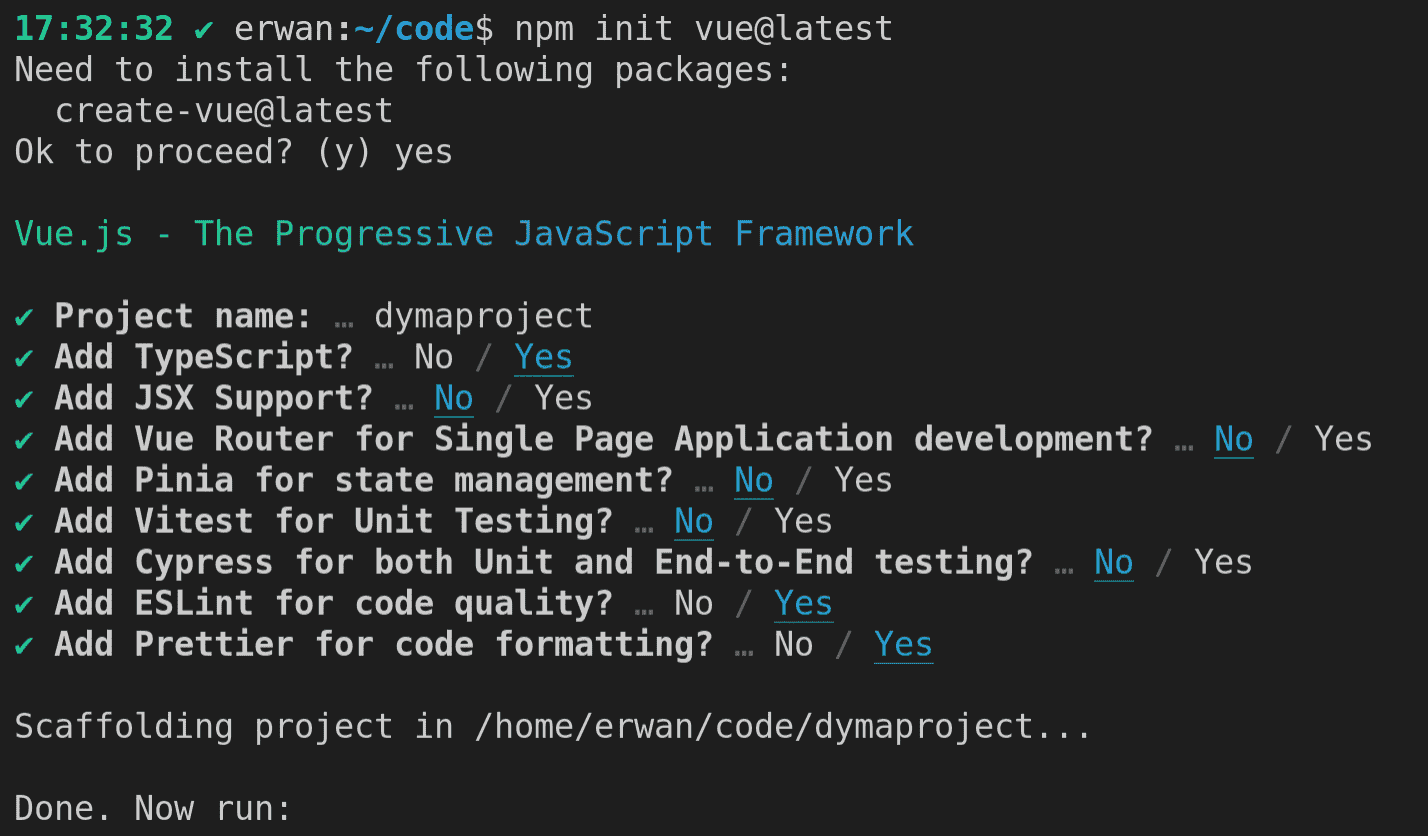
\includegraphics[width=10cm]{images/image04.png}
\end{center}



\end{document}

